\begin{figure}[!b]
    \centering
    \begin{subfigure}[b]{0.48\textwidth}
        \centering
         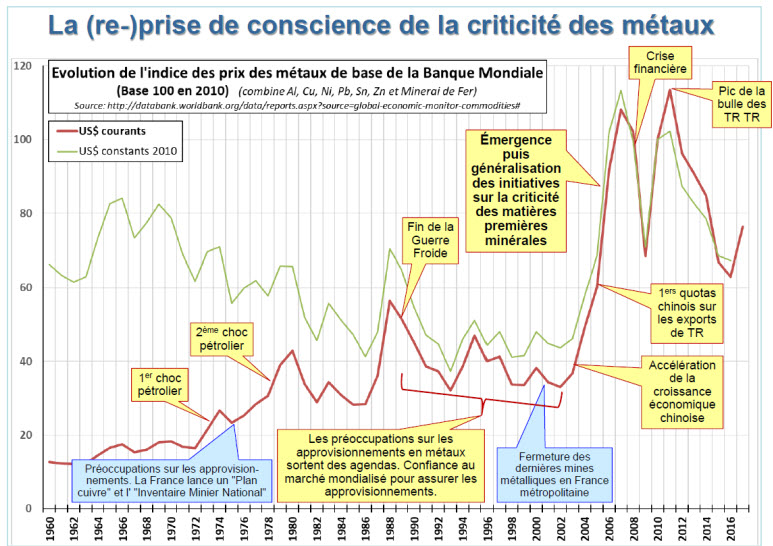
\includegraphics[width=\textwidth]{Images/Metals_policies/indice_metal.jpg}
         \caption{Indice des prix des métaux (\cite{brgm_substances_2022})}
         \label{fig:indices_metal}
    \end{subfigure}
    \hfill
    \begin{subfigure}[b]{0.48\textwidth}
        \centering
         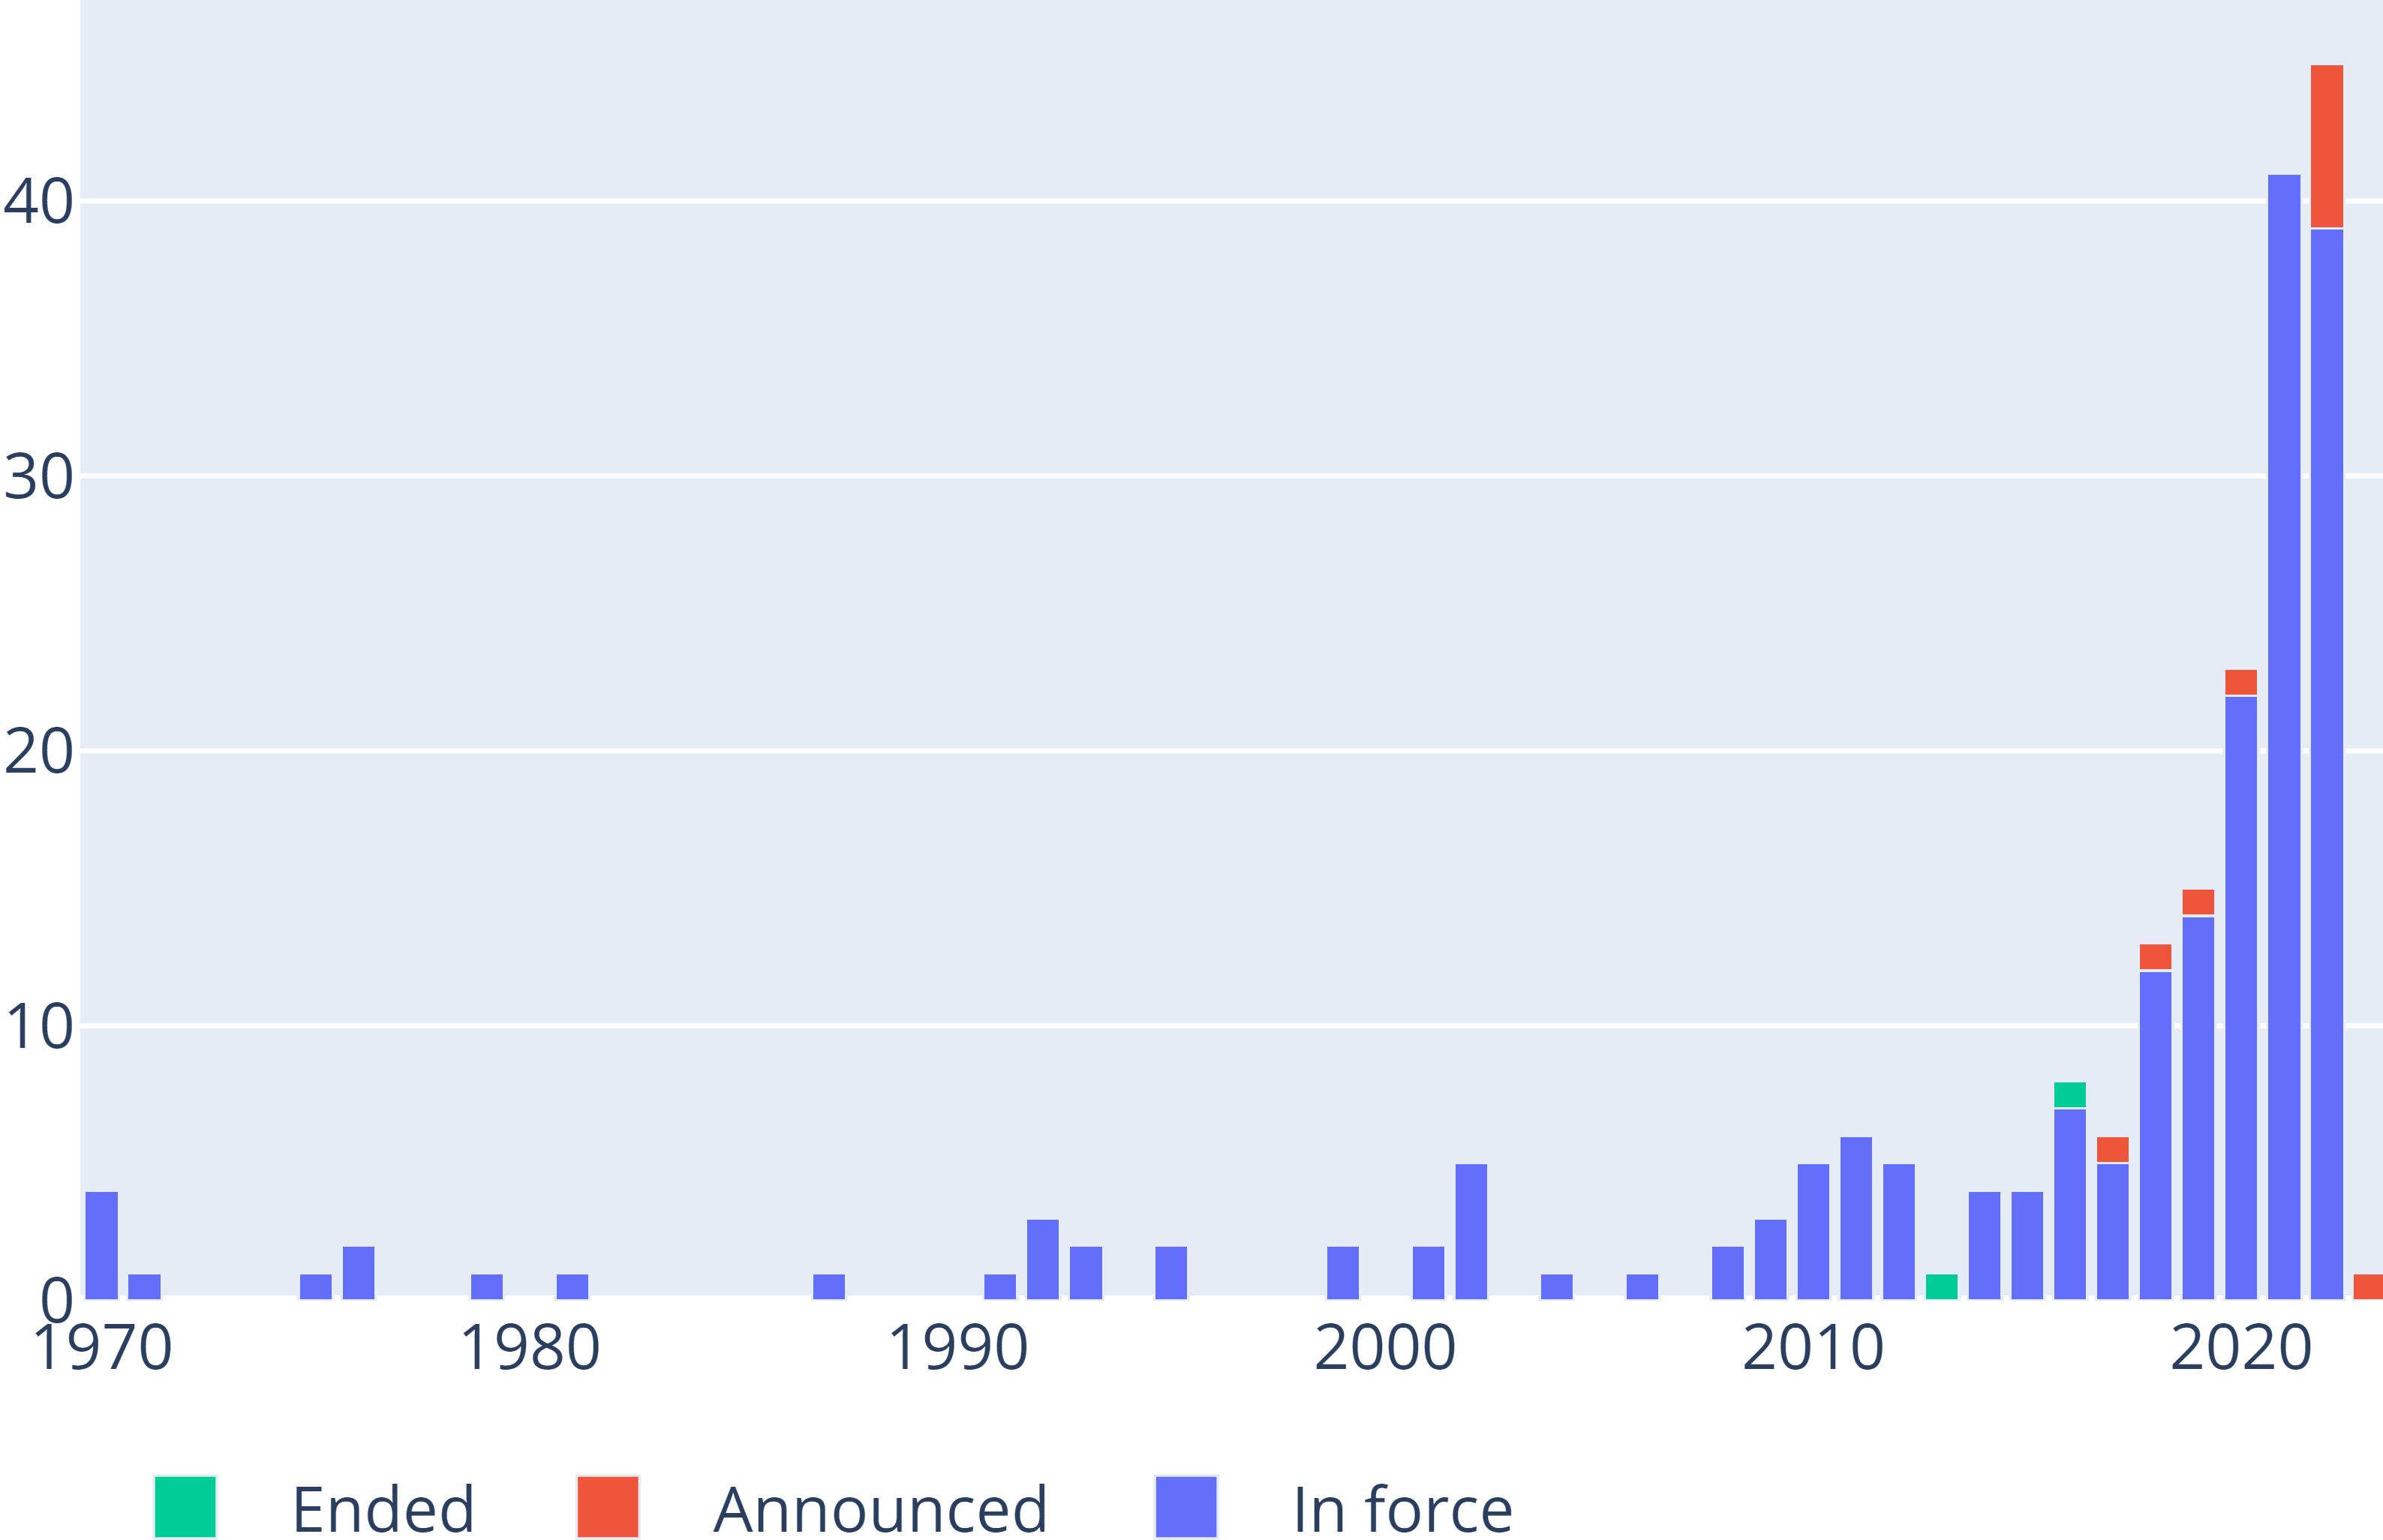
\includegraphics[width=\textwidth]{Images/Metals_policies/critical_metals_policies.png}
         \caption{Politiques publiques sur les métaux critiques (\cite{iea_critical_2022})}
         \label{fig:politiques_metal}
    \end{subfigure}
    \caption{Tendances historiques sur les métaux}
    \label{fig:metal_histoire}
\end{figure}
Les sections précédentes ont permis d'exposer certains risques géopolitiques pouvant être exacerbés par la décarbonation des mix énergétiques. Pour compléter cette étude, cette section propose une revue des politiques publiques sur les matériaux critiques dans le monde. L'objectif est d'apporter des éléments sur le caractère maîtrisable de ces risques géopolitiques.\smallbreak
L'approvisionnement en métaux est historiquement un enjeu militaire. La Guerre froide a engendré une course à l'armement et à l'espace, les industries militaires avaient alors le quasi-monopole de l'usages des métaux rares (\cite{donnen_vers_2022}). En 1950, le Congrès américain a adopté le \textit{'Defense Production Act'} pour conférer au président les pouvoirs nécessaires afin d'assurer l'approvisionnement en matériaux et les services nécessaires à la défense nationale, renonçant parfois aux exigences du commerce international. Initialement adoptée pour assurer la disponibilité du matériel de défense militaire pendant la guerre de Corée, le président Biden l'a invoquée pour sécuriser la production de vaccins COVID-19 en janvier 2021 et la production de lances à incendie en septembre 2021, afin d'atténuer les effets des incendies de forêt dans tout le pays (\cite{iea_critical_2022}).\smallbreak
La fin de la guerre froide a engendré une forte baisse des tensions sur l'approvisionnement avec d'une part la baisse de la demande des industries militaires et d'autre part la hausse de l'offre de la part des pays du bloc de l'Est. Cette relaxation a eu pour conséquence une diminution des prix des métaux (figure \ref{fig:indices_metal}) et une diminution des politiques publiques pour la sécurisation des approvisionnements en métaux. En France, la Caisse française des matières premières (CFMP) est dissoute en 1997. Elle assurait depuis 1980 la constition d'un stock stratégique de matières premières (\cite{donnen_vers_2022}).\smallbreak
A partir des années 2000, la croissance économique chinoise et la digitalisation de l'économie rendirent les chaînes d'approvisionnement à nouveau critiques. Cette tendance est amenée à s'amplifier avec les objectifs de décarbonation des pays du monde. La prise de conscience est visible à travers le nombre de politiques publiques sur les métaux critiques ces dernières années (figure \ref{fig:politiques_metal})\smallbreak
Cette section analyse les politiques publiques sur les chaînes d'approvisionnement en quatre parties. La première partie porte sur l'identification des faiblesses d'approvisionnement et leur importance par les politiques publiques. Les chaînes d'approvisonnement et les technologies bas-carbone étant complexes, l'identification et la quantification des risques est difficile. La deuxième partie porte sur les politiques publiques pour l'amélioration de la fiabilité des approvisionnements. La criticité des chaînes d'approvisionnement étant posée en première partie, la seconde partie développe les moyens de faire face à ces faiblesses. La troisième partie porte sur la maîtrise des chaînes de valeur. Cette partie se concentre plus sur la partie aval des deux parties précédentes, en abordant l'innovation et le recyclage. Enfin, la quatrième partie porte la durabilité de l'approvisionnement. En cohérence avec la décarbonation, une chaîne d'approvisionnement durable est bas-carbone. Le respect de normes environnementales et sociales des chaînes d'approvisionnement en augmenteront la fiabilité sur le long terme. 

